\chapter{Implementation}
\section{ADT}
The SearchTreeNode() can be represented as an ADT with six instance variables. The \textbf{state} of the state space that this node corresponds to, the \textbf{parent node}, implemented by the same ADT, the \textbf{operator} applied to generate this node, the \textbf{depth} of the node in the tree, the \textbf{path cost} from the root and the \textbf{Heuristic} value of the node.\\

The SearchProblem() ADT is characterized by the following variables. The \textbf{State Space} containing all states reachable by any sequence of actions, the \textbf{initial state}, and list of \textbf{operators} available for the agent. Moreover, the goal test is computed by the function \textbf{boolean goalTest(State state)}, that takes a state as a parameter and checks if all parts are assembled or not. Also, it calculates the \textbf{pathcost(Objects... actions)} $412312$%!@3.

Where-are-my-parts ADT is the main class that calls genGrid() to generate a grid, calls the search() method to find the solution by calling a method for every Search Algorithm implemented inside the class. 

\section{Main Functions}
\subsubsection{GetBulkRec}
GetBulkRec(Part p) is a function that returns all the Parts attached to the current part p and all the parts attached to them recursively . For simplicity, it gets all parts attached in a bulk if Part P is a subset of this bulk.



\subsubsection{Transfer function}

\subsubsection{Fix}


\chapter{Algorithms}
\section{Implementation}
\subsubsection{Breadth First Search}

A to-be-expanded queue is initialized at the beginning of the search approach, and the BFS function is called whenever this queue is nonempty. The function dequeues the first node from the beginning of the queue, expand it, and adds the expanded nodes to the end of the queue, till the goal test is satisfied or there is no solution ( empty queue).

A simple adjustment to the algorithm has been implemented, as the repeated identical nodes are removed from the queue, due to the fact that the children would be identical as well, thus creating redundant sub-problems. ( similar to the divide-and-conquer concept)

\subsubsection{Depth First Search}

A to-be-expanded queue is initialized at the beginning of the search approach, and the DFS function is called whenever this queue is nonempty. The function dequeues the first node from the beginning of the queue, expand it, and adds the expanded nodes to the beginning of the queue, till the goal test is satisfied or there is no solution ( empty queue). 


\subsubsection{Iterative Deepening Search}

Iterative deepening simply sets a limit for the DFS function, thus, a limit is set at the beginning of the search, and the DFS function is called till the limit is reached, the goal test is satisfied or the queue get emptied.

\subsubsection{Greedy Search}
Greedy Search is set to expand the least heuristic valued node in the global queue of expanded nodes. Thus, the search dequeues the first value in the queue, expand it, and sort the children according to the heuristic value using insertion sort. It terminates if the goal test is achieved or the queue get emptied. However, due to the nature of the Where-are-my-parts problem, Robots can keep hitting an obstacle forever. This incompleteness gives the Greedy search an non-terminating manner in most cases.

\subsubsection{A* Search}
The A* Search follows the same footsteps of the greedy. However, it takes to account the number of steps moved so far from the root node up to the current node as a part of the priority value in the queue. Thus, giving greedy search a completeness feature. i.e, a node with a robot hitting the wall will increase his priority queue value, putting it a step back for another node to try its luck.

\section{Comparison}

As shown in graph \ref{fig:graph}, only Breadth-First, Iterative Deepening and A* search algorithms made it through the test cases due to its completeness feature.  The A* search hold the least number of expanded nodes, which shows how precise is the heuristic (will be explained later), followed by the Iterative Deepening search, and finally the Breadth-first Search.

\begin{figure}[H] 
   	\centering
	\includegraphics[scale=0.6]{images/Graph} 
    \caption{Implemented Algorithms vs Number of expanded nodes. (1000 represent infinity}
    \label{fig:graph} 
\end{figure}




\chapter{Heuristic}
\section{Centroid}

The Centroid approach was used and implemented as a heuristic function in the project. As in, The heuristic function returns the average distance between the robot parts in the grid and the centroid point between them. As illustrated in figure \ref{fig:centroid_model}, every robot parts' X and Y coordinates are modeled as a point in the grid. The points are used to create a virtual polygon by the aid of the geometry library "JTS". The Centroid is calculated using Polygon.getCentroid() function from JTS library. Finally, the average distance between all points and the centroid is returned as the heuristic value.

\begin{figure}[H] 
   	\centering
	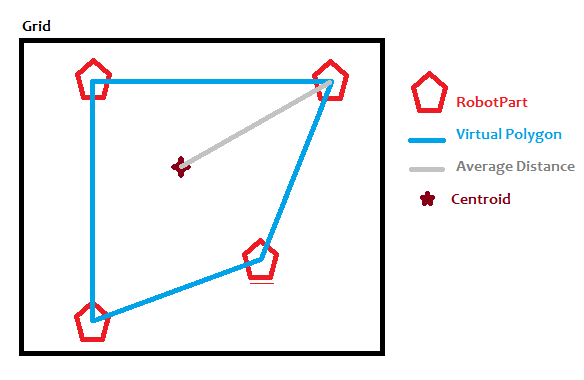
\includegraphics[scale=0.6]{images/Centroid} 
    \caption{Centroid concept illustration}
    \label{fig:centroid_model} 
\end{figure}

The heuristic approach proved to be a successful one, however it had a major drawback. If the Centroid can't be calculated because of the nature of the irregular shape e.g A twisted polygon as shown in figure \ref{fig:twistedcentroid}. The heuristic will return infinity. which wasn't acceptable. 

\begin{figure}[H] 
   	\centering
	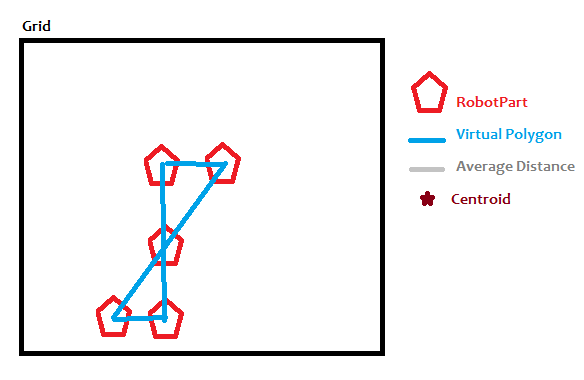
\includegraphics[scale=0.6]{images/twistedcentroid} 
    \caption{Centroid is incalculable incase of twisted polygons. }
    \label{fig:twistedcentroid} 
\end{figure}


\section{Average Distances}

Due to the Centroid unsuccessful attempt, the Average Distances approach was used. As in, it gets the summation of all the distances between all parts and each others as shown in figure \ref{fig:averagedistance}. The result is divided on the number of the parts Squared, to get an admissible Average Heuristic.

\begin{figure}[H] 
   	\centering
	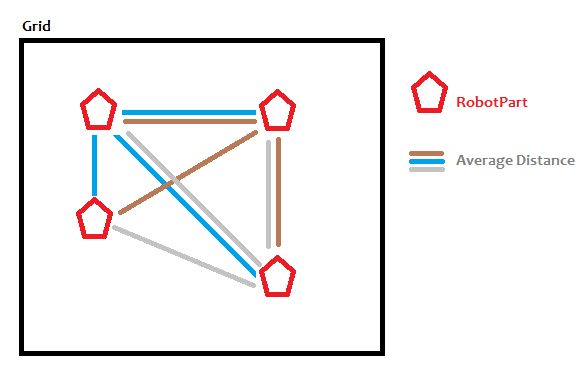
\includegraphics[scale=0.6]{images/averagedistance} 
    \caption{The distances between all parts and each other is used to evaluate the average distance. }
    \label{fig:averagedistance} 
\end{figure}

The heuristic approach is satisfying the \textbf{Centering} property. The heuristic function will check for merged up parts, returning a zero when all parts are conjoined, and returning the Average distance otherwise. \\

The approach followed is \textbf{consistent}. The heuristic value increases if one the parts stray away from the others, and decreases when it gains on other parts. The averaging is designed to get the Sum of distances and divide on the Number of parts squared. Thus, avoiding any chance for any overestimation of heuristic. Moreover, parts move in 2D grid, the average distance between 2 parts in a grid is the hypotenuse in most cases, which is always shorter than the catheti. and in case of straight lines, the distance is the same as the heuristic value (assuming distance is in unit steps), which proves \textbf{admissibility}.	


\section{Number of Bulks remaining}

The Number of Bulks remaining heuristic is a simple approach mainly used to assemble parts as fast as possible, The main concept is calculating the number of combined bulks of robot parts represented in the grid. Give more priority for small bulks to move, thus aiming to decrease the path cost by not moving the huge bulks to the smaller ones. Also, it gives more priority for parts merging into other parts, rather than stopping at an obstacle.  \\

The heuristic function is calculated as follows, the size of the bulks in the grid is doubled and added. Thus, bigger bulks will have larger output. The output is inversed to satisfy the \textbf{Monotonic} property by giving the bigger bulks less heuristic values. The function returns the number of parts in the board divided by the inversed value to satisfy the \textbf{admissibility} property. Finally, The \textbf{Centering} property is satisfied by a running check, returning a zero value if the number of bulks reaches one, i.e, there is only 1 merged robot.


\chapter{External Libraries}

The JTS Topology Suite is an opensource API of 2D spatial predicates and functions. JTS geometry library was used in the project to implement the Centroid and Average Distances Heuristics. \\

 Centroid was calculated as follows, every Robot Part's coordinates creates a new JTS \textbf{coordinates(double x,double y)}, which its used as a parameter for a \textbf{linearRing(Coordinates[] s)}, that creates the virtual \textbf{polygon(LinearRing r)}, the Centroid can be easily calculated using \textbf{Polygon.getCentroid()} which returns the centroid as a Point.\\
 
 Average Distances was calculated simply by using the following line, \textbf{DistanceOp.distance(Point x,Point y)}, where Point takes Coordinate as a parameter. Returns the average distance between two given points.
 \\
 
 
 